\chapter[Introdução]{Introdução}
\label{cap:introducao}

Atualmente, existe uma grande procura por funcionários especializados em Tecnologia da Informação (TI) e áreas similares, sendo percebida no mundo todo uma grande carência de profissionais qualificados para atuar nessas áreas.
Apesar do grande crescimento nas áreas de STEM (Science, Technology, Engineering and Mathematics) [Ciência, Tecnologia, Engenharia e Matemática], o número de profissionais qualificados nessas áreas não acompanha esse crescimento e a perspectiva é de que essa situação se acentue ainda mais no futuro \cite{shortage_of_workers}.

Devido a essa carência de profissionais, torna-se importante a busca por formas de incentivar o aprendizado e a busca por conhecimento por parte dos jovens.
Visando solucionar esse problema, foi decidido realizar um trabalho que incorpore conceitos de robótica, já que seu uso em atividades com crianças consegue influenciar positivamente o desenvolvimento de habilidades da área de STEM, conforme estudos realizados nos Estados Unidos e Europa \cite{technology_for_stem}, e projetos desenvolvidos no Brasil \cite{robotica_educacao}.

Com base nisso, foi proposto realizar o desenvolvimento de uma plataforma que utilize recursos computacionais passível de ser utilizada para demonstrar conceitos nas áreas de computação, elétrica e controle.
Para aumentar o interesse por esta plataforma foi decidido incorporar um jogo de tabuleiro no projeto e foi escolhido o Xadrez, por ser um jogo que exige raciocínio lógico e estratégico, além de ser popular e bastante conhecido.
Correlacionando ambas essas ideias, implementou-se um jogo de Xadrez que pode ser jogado utilizando-se braços robóticos, similar ao que é mostrado na Figura \ref{fig:bracoRoboticoXadrez}.

\begin{figure}[H]
    \centering
    \caption{Braço Robótico com peças de Xadrez}
    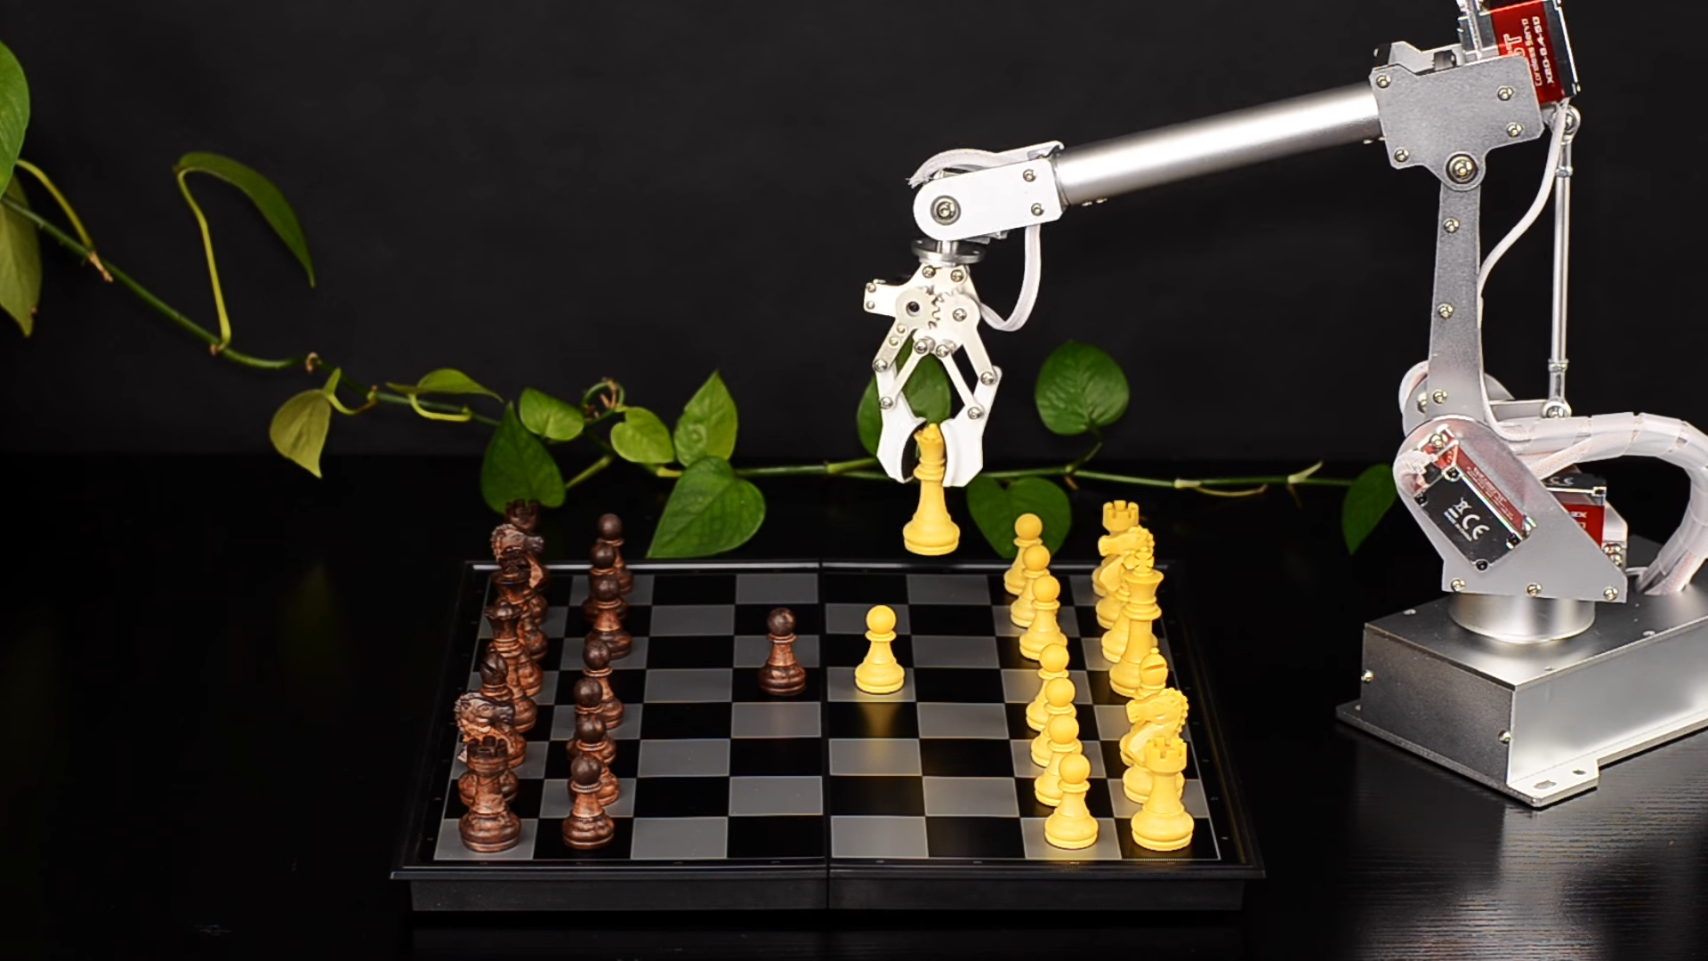
\includegraphics[keepaspectratio=true, width=0.8\textwidth]
    	{img/robotic-arm-chess-example.png}
    \fonte{\url{https://www.youtube.com/watch?v=OHazT3y0WpI}}
    \label{fig:bracoRoboticoXadrez}
\end{figure}

No Capítulo \ref{cap:trabalhosRelacionados} serão apresentados alguns trabalhos que apresentam características semelhantes ao que foi proposto e foram utilizados como base para o desenvolvimento deste trabalho.
Em seguida, no Capítulo \ref{cap:metodologia} será apresentada a metodologia utilizada para o desenvolvimento do trabalho.
No Capítulo \ref{cap:planejamento} será apresentado um resumo sobre as regras do xadrez e o planejamento do projeto, incluindo a definição dos componentes utilizados e a forma de integração entre eles.
Posteriormente, no Capítulo \ref{cap:desenvolvimento} será apresentado o desenvolvimento do projeto e uma análise de seu desempenho, incluindo a montagem dos componentes físicos, e o desenvolvimento dos \textit{softwares} utilizados.
Por fim, no Capítulo \ref{cap:conclusao} serão apresentadas as conclusões obtidas com o desenvolvimento do projeto e sugestões para trabalhos futuros.